This section depicts the Gibbs energy surfaces predicted using the model parameters calculated from ternary liquid-liquid equilibrium data. The two experimental tie-lines, used for the pseudo-analytical method of parameter estimation, are indicated as solid black lines. In the figures that follow, regions where the Hessian matrix of the Gibbs energy function is not positive definite, i.~e. where the ternary mixture is unstable, are projected below the  Gibbs energy surface and indicated in red.\\

%%------------------------------- Cyclohexane, Benzene and Nitro-Methane-------------------------------------------%
\subsection{Cyclohexane, Benzene and Nitro-Methane}

\begin{figure}[hp]
 \vspace{40pt}
\centering
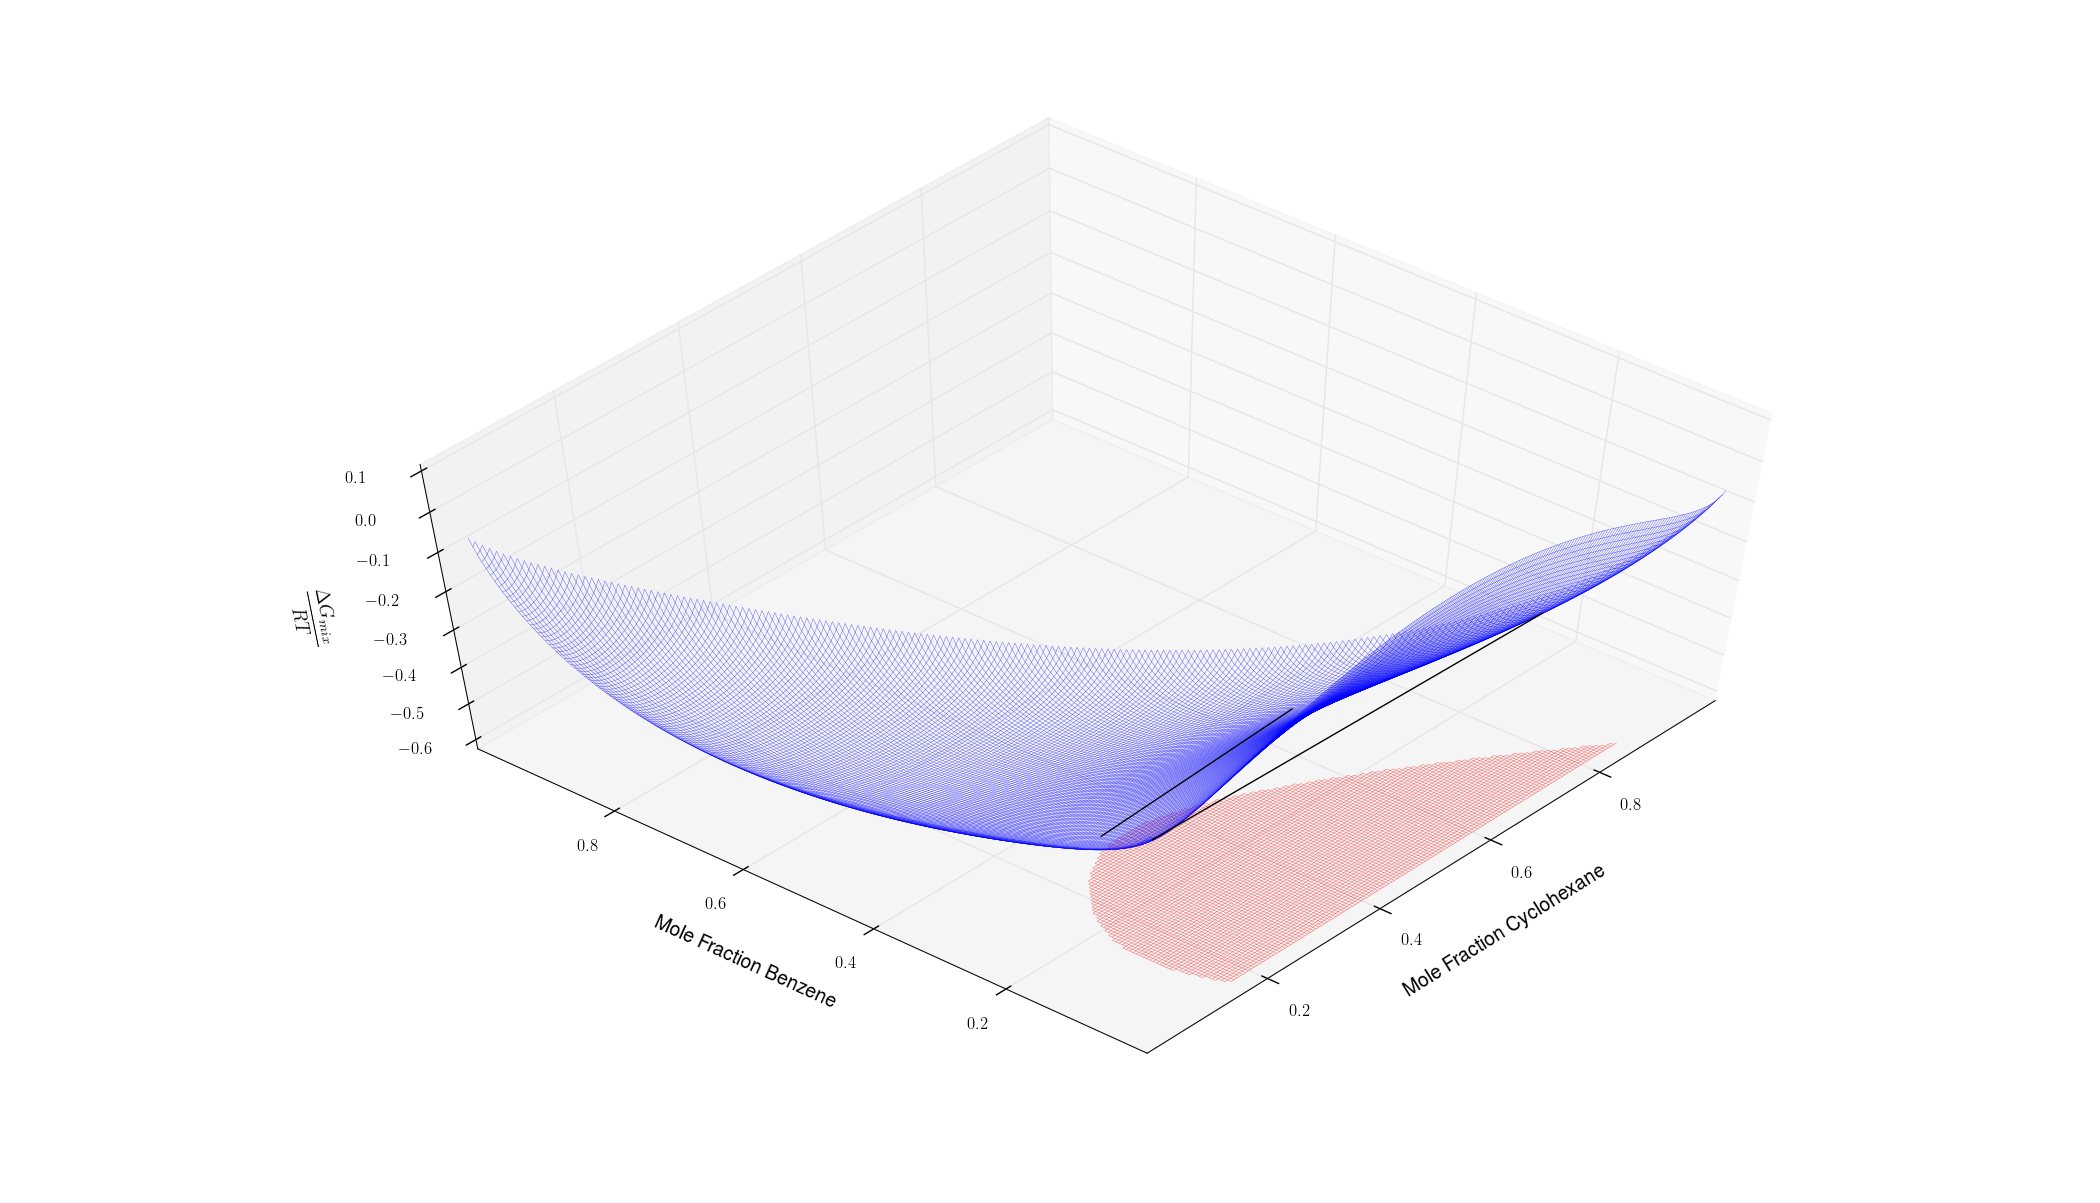
\includegraphics[width = \textwidth, bb=100 100 1600 700]{Results_Parts/TernaryParams/cyclohexane-benzene-methanenitro/DWPM/rotation1.png}
\caption{Predicted Gibbs energy surface for Cyclohexane, Benzene and Nitro-Methane at $298.15~\mathrm{K}$}
\end{figure}	

\begin{figure}[hp]
\vspace{40pt}
\ContinuedFloat
\centering
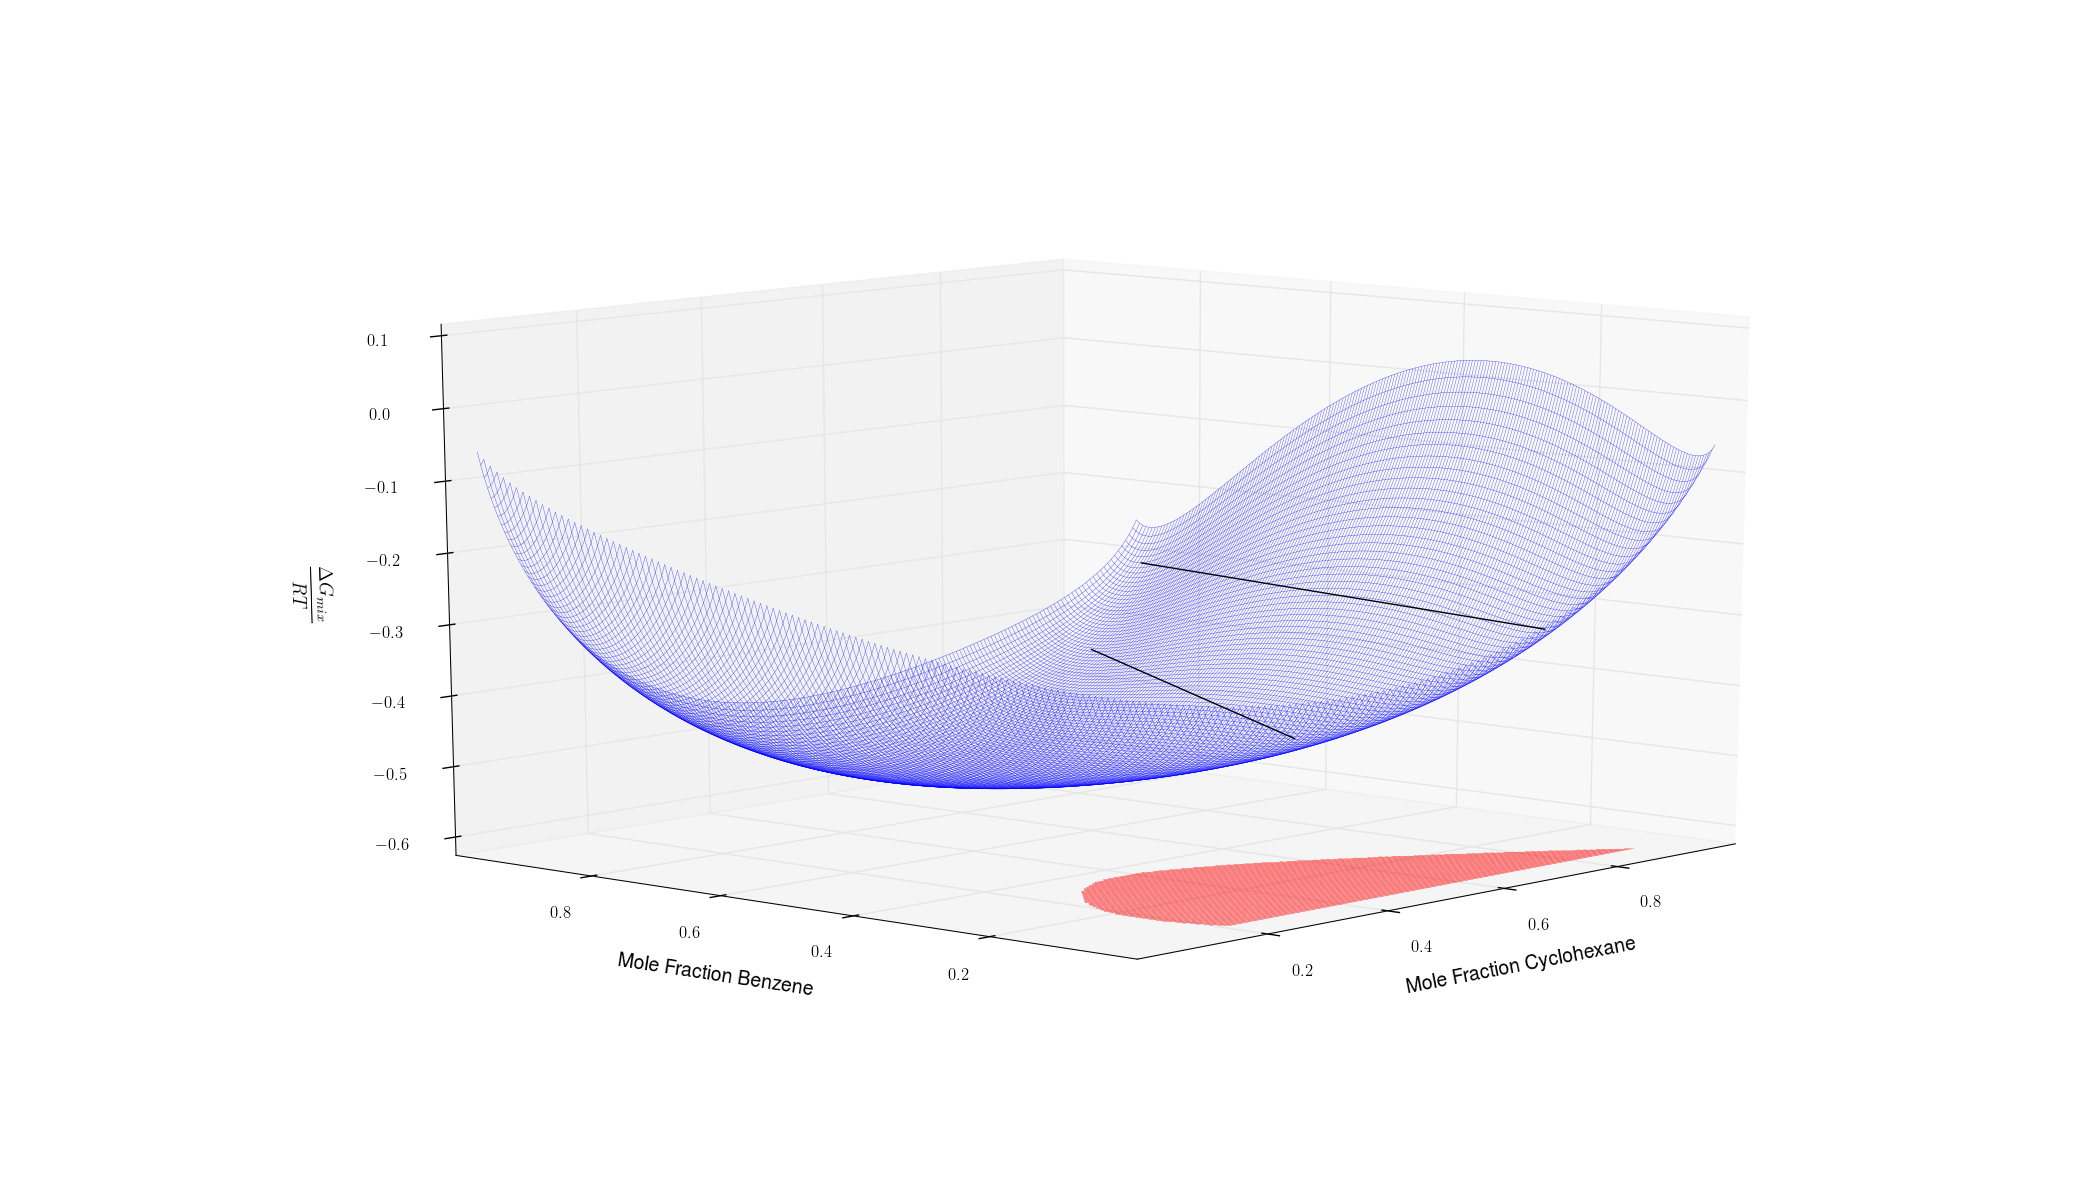
\includegraphics[width = \textwidth, bb=100 100 1600 700]{Results_Parts/TernaryParams/cyclohexane-benzene-methanenitro/DWPM/rotation2.png}
\caption[]{(Continued) Rotated View 1}
\end{figure}

\begin{figure}[hp]
\vspace{40pt}
\ContinuedFloat
\centering
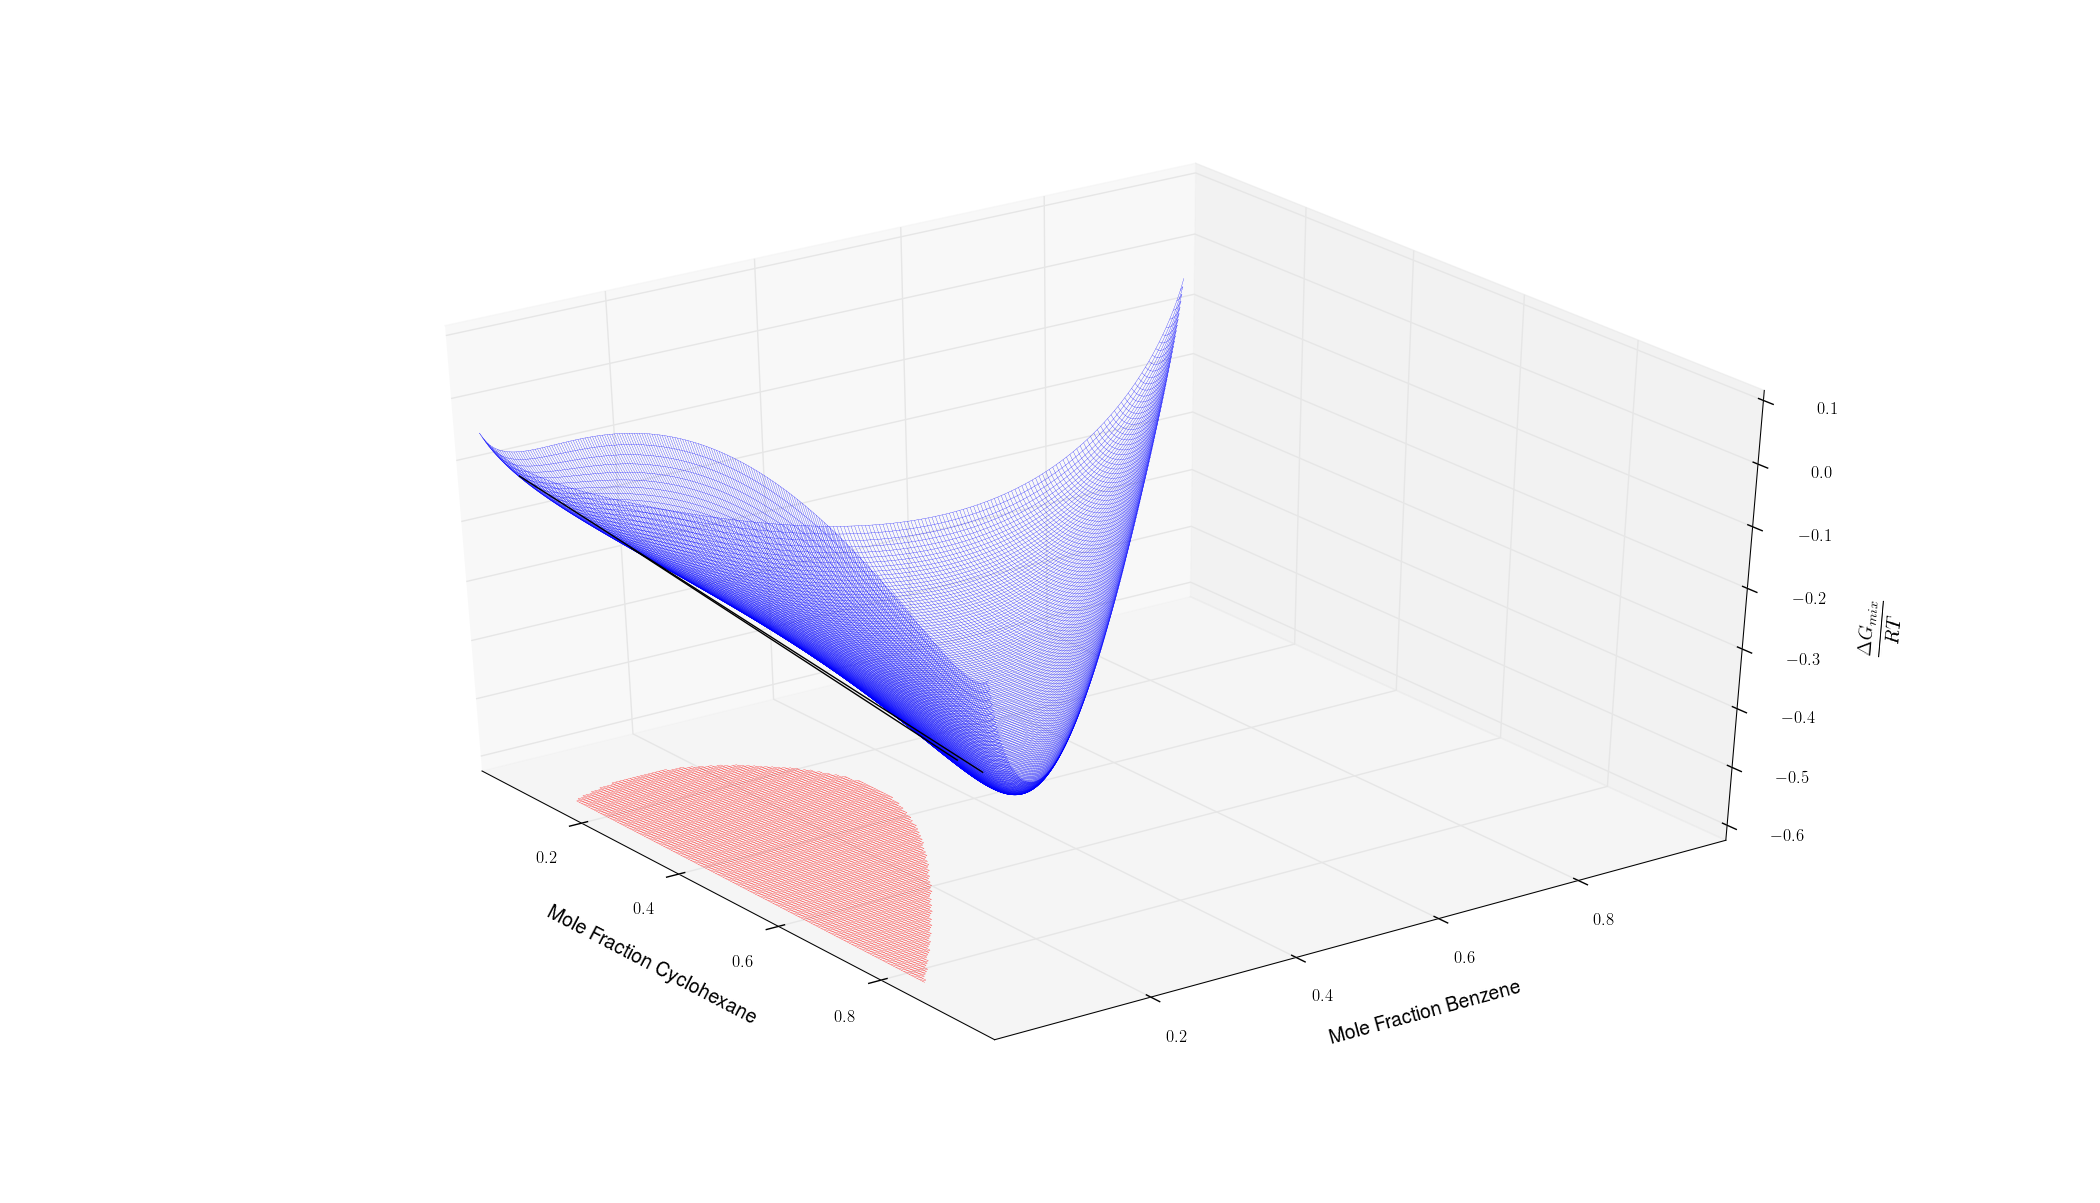
\includegraphics[width = \textwidth, bb=100 100 1600 700]{Results_Parts/TernaryParams/cyclohexane-benzene-methanenitro/DWPM/rotation5.png}
\caption[]{(Continued) Rotated View 2}
\end{figure}

\begin{figure}[hp]
\vspace{40pt}
\ContinuedFloat
\centering
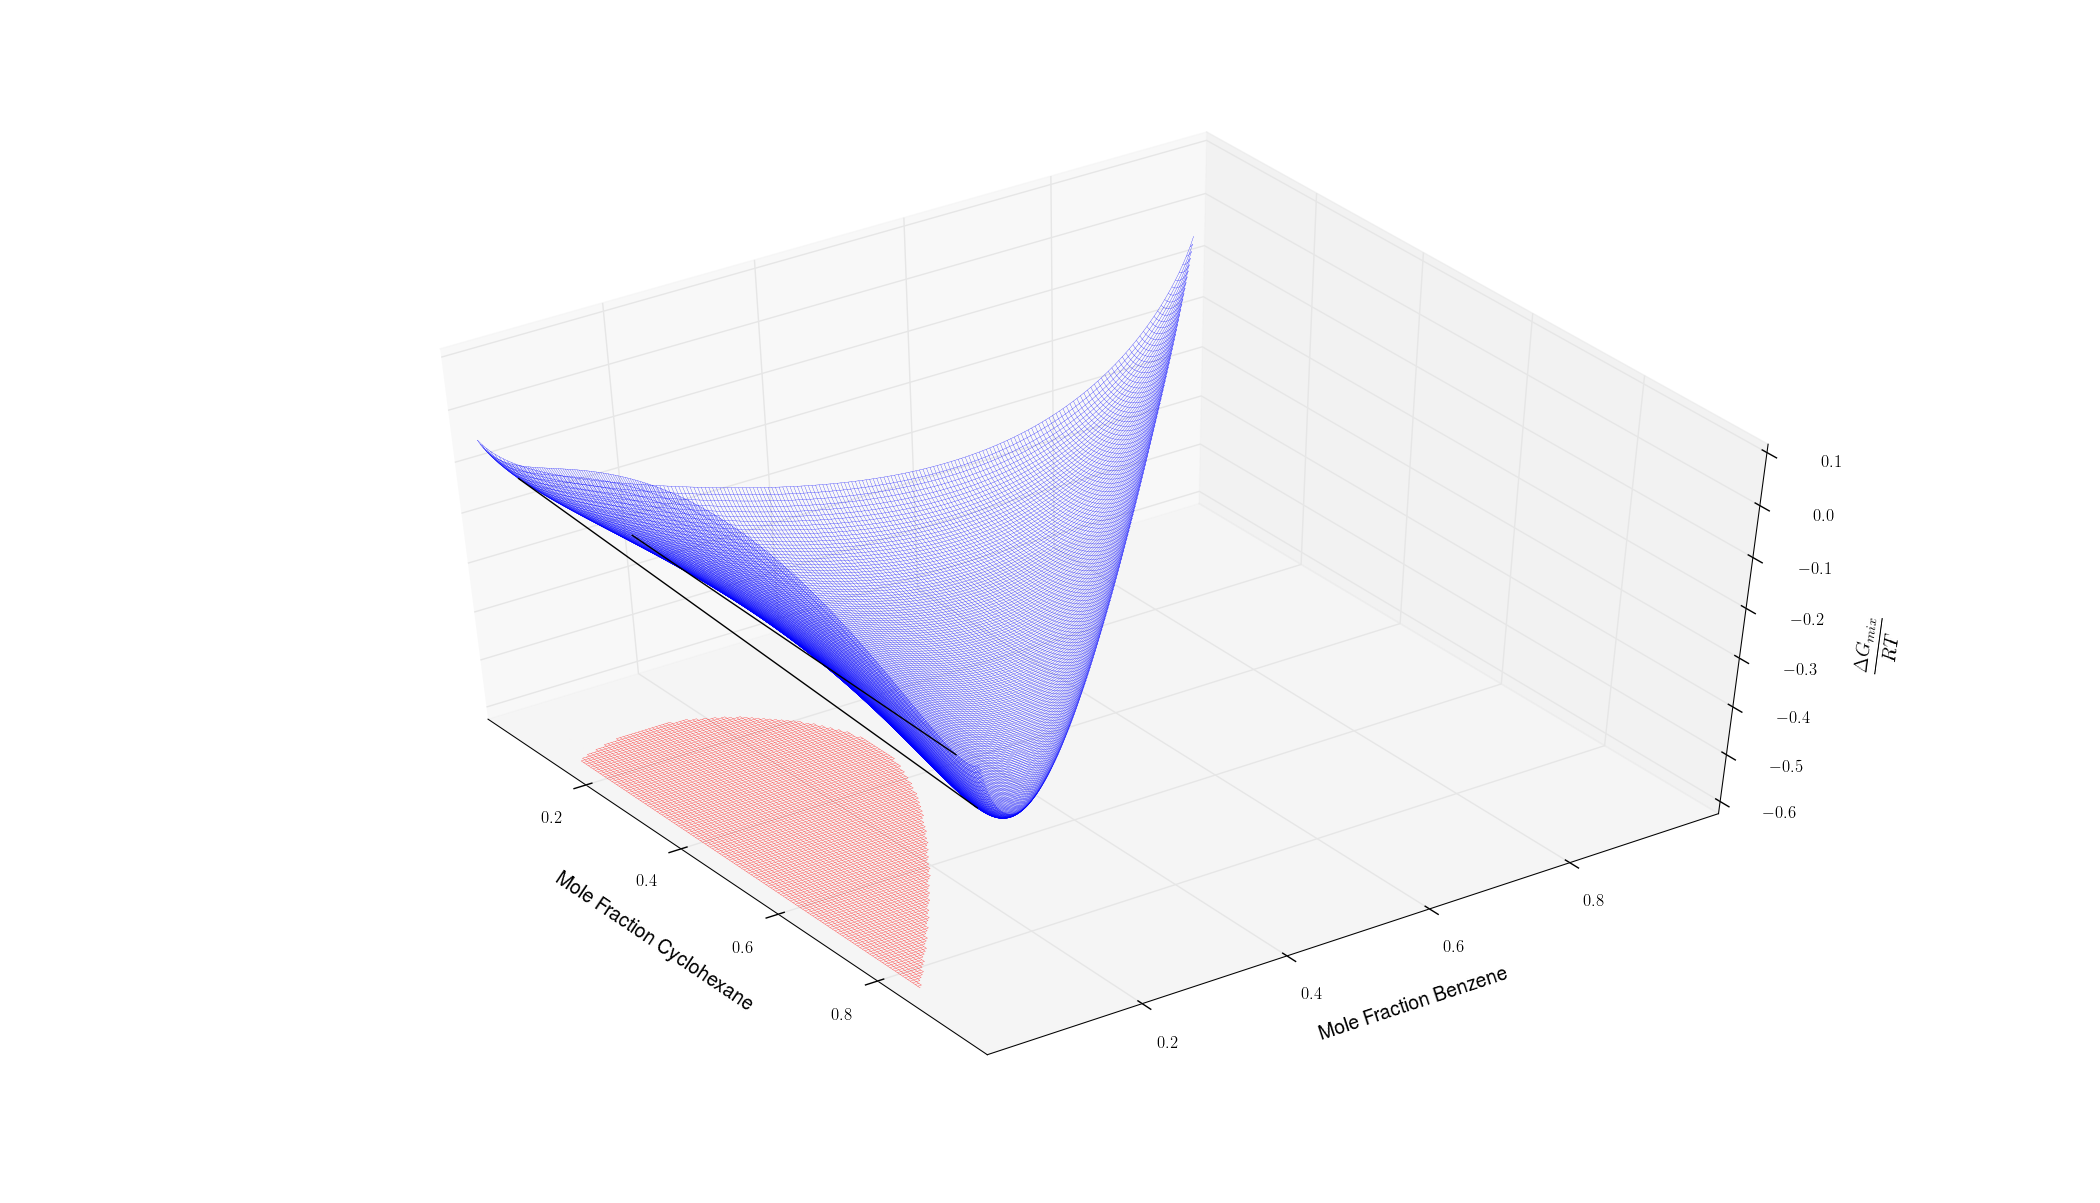
\includegraphics[width = \textwidth, bb=100 100 1600 700]{Results_Parts/TernaryParams/cyclohexane-benzene-methanenitro/DWPM/rotation6.png}
\caption[]{(Continued) Rotated View 3}
\end{figure}
\clearpage

%%------------------------------- Heptane, Hexane and Methanol-------------------------------------------%
\subsection{Heptane, Hexane and Methanol}

\begin{figure}[hp]
 \vspace{40pt}
\centering
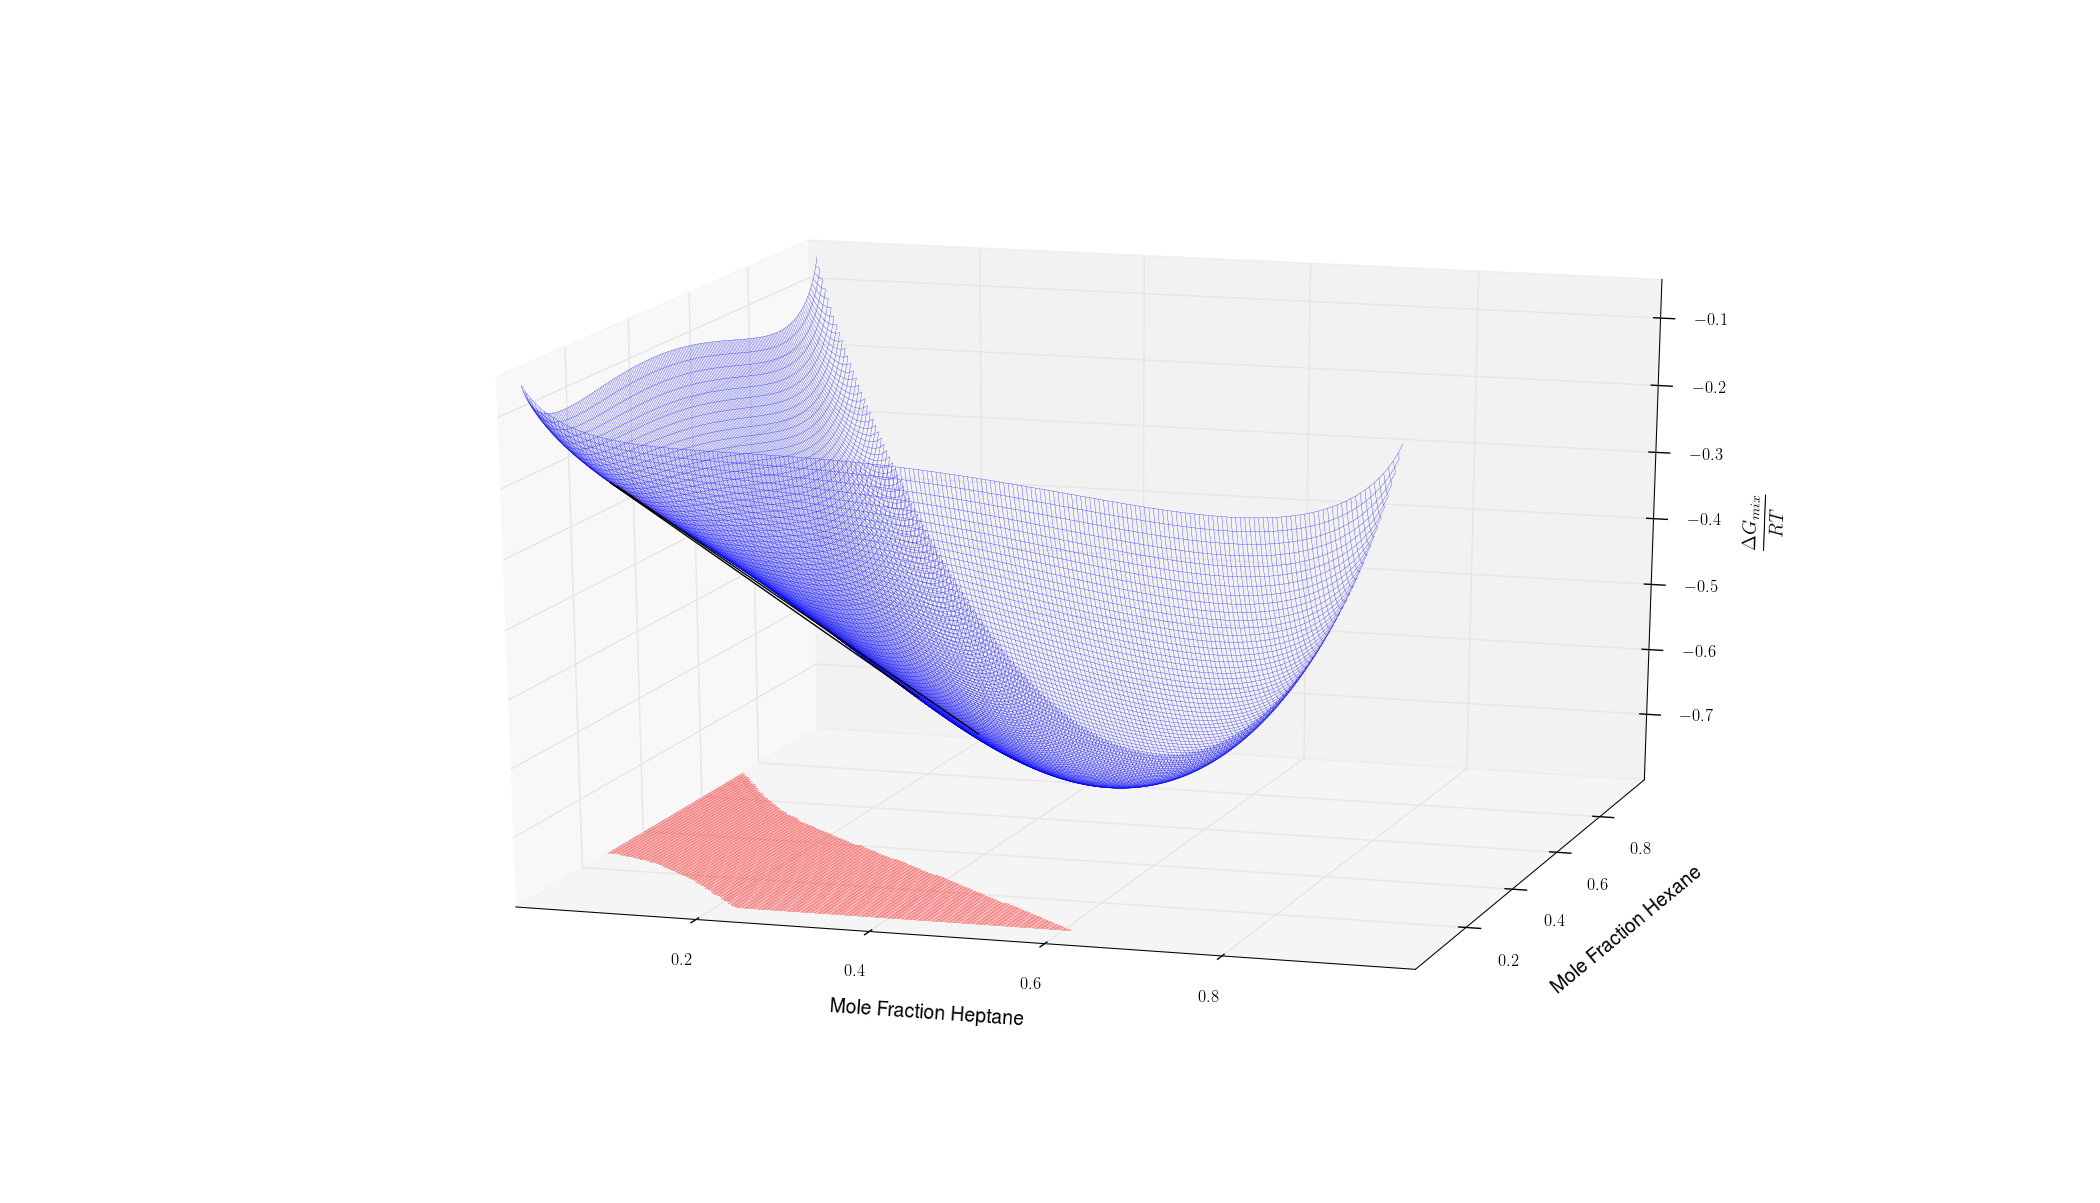
\includegraphics[width = \textwidth, bb=100 100 1600 700]{Results_Parts/TernaryParams/heptane-hexane-methanol/DWPMTieline3and4/rotation4.png}
\caption{Predicted Gibbs energy surface for Heptane, Hexane and Methanol at $305.95~\mathrm{K}$, using parameters calculated from experimental tie-lines 3 and 4.}
\end{figure}	

\begin{figure}[hp]
\vspace{40pt}
\ContinuedFloat
\centering
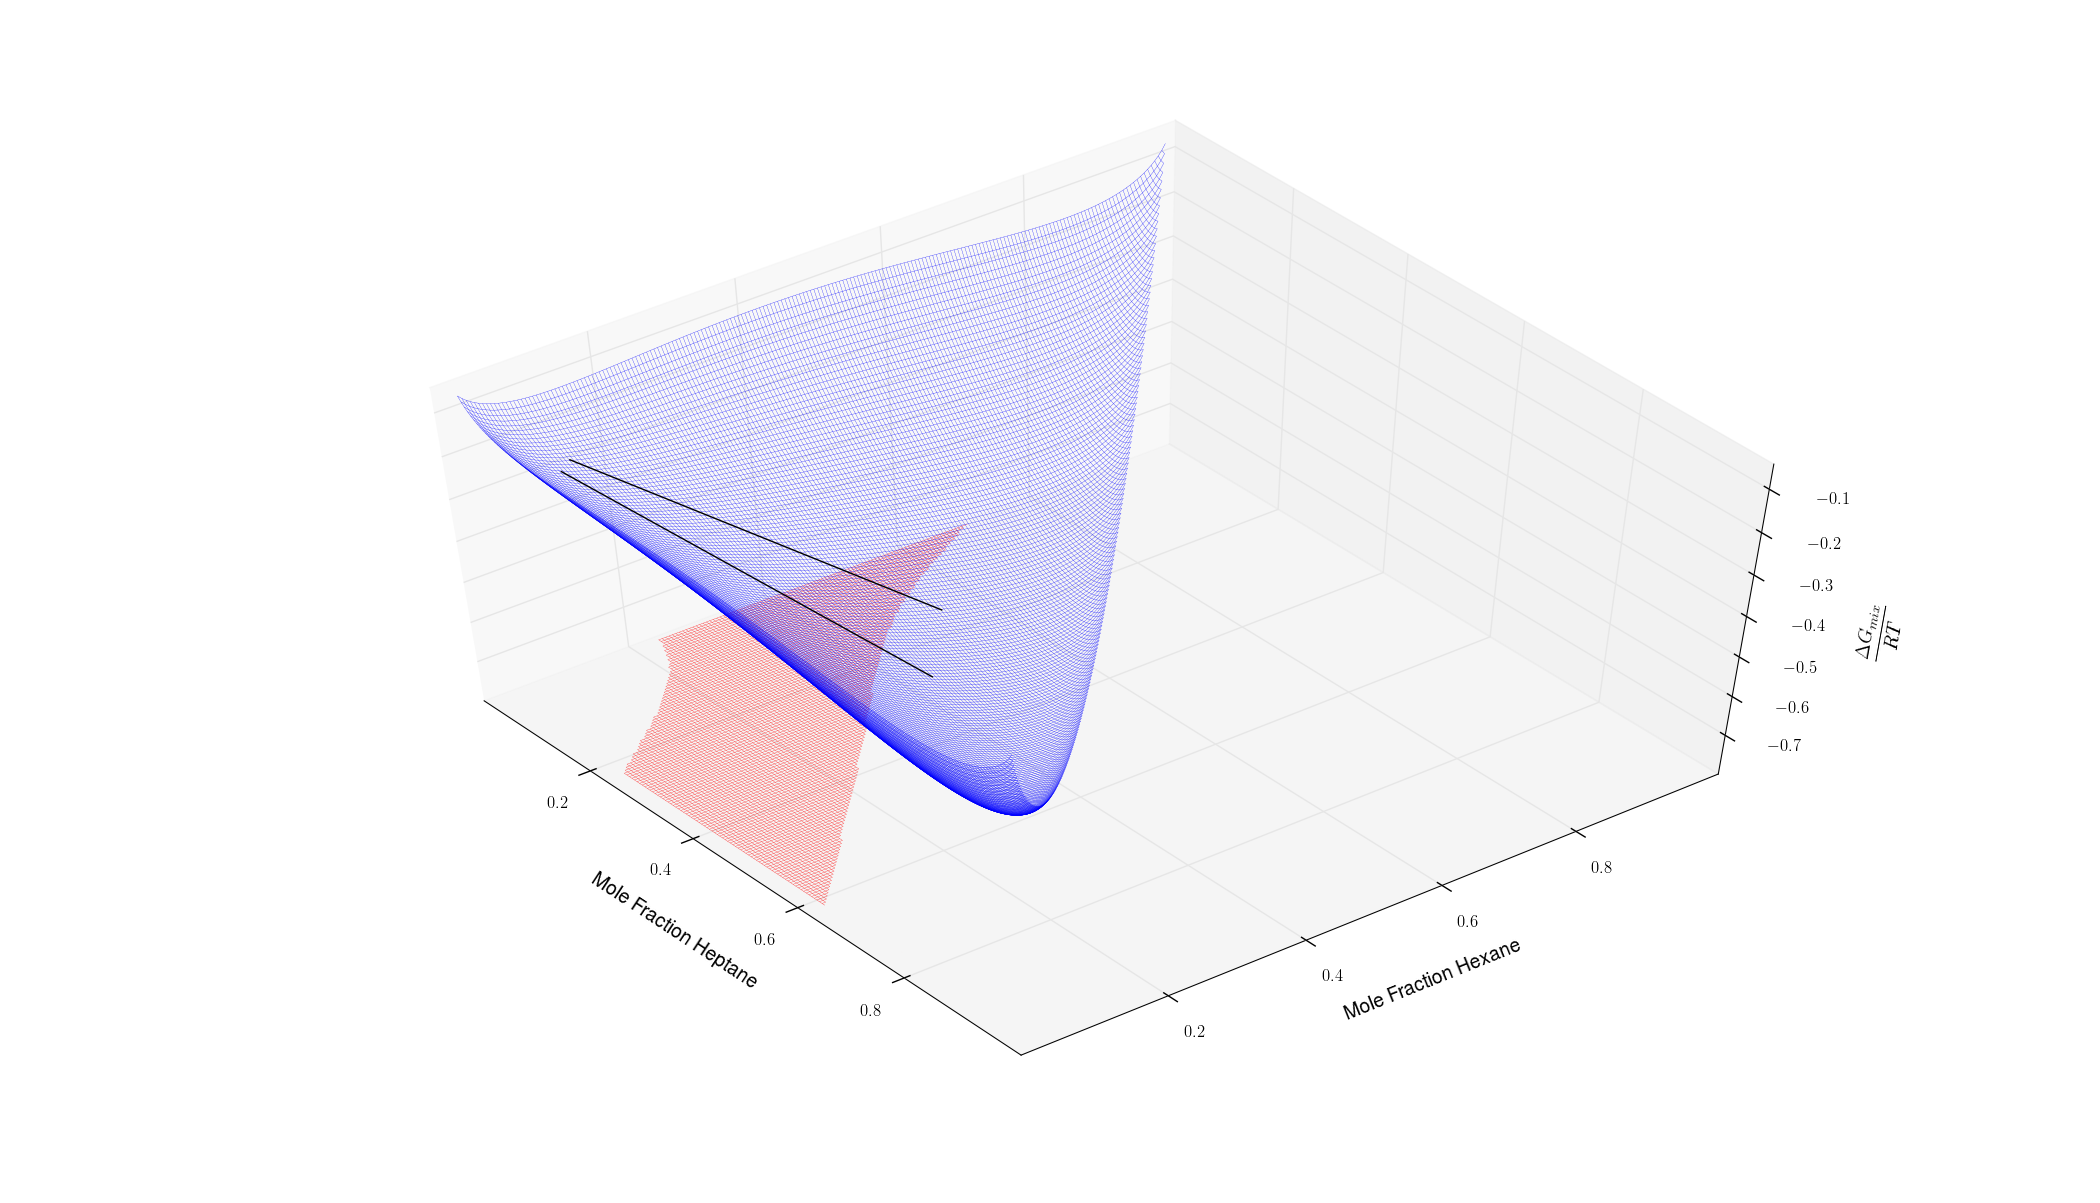
\includegraphics[width = \textwidth, bb=100 100 1600 700]{Results_Parts/TernaryParams/heptane-hexane-methanol/DWPMTieline3and4/rotation3.png}
\caption[]{(Continued) Rotated View 1}
\end{figure}

\begin{figure}[hp]
\vspace{40pt}
\ContinuedFloat
\centering
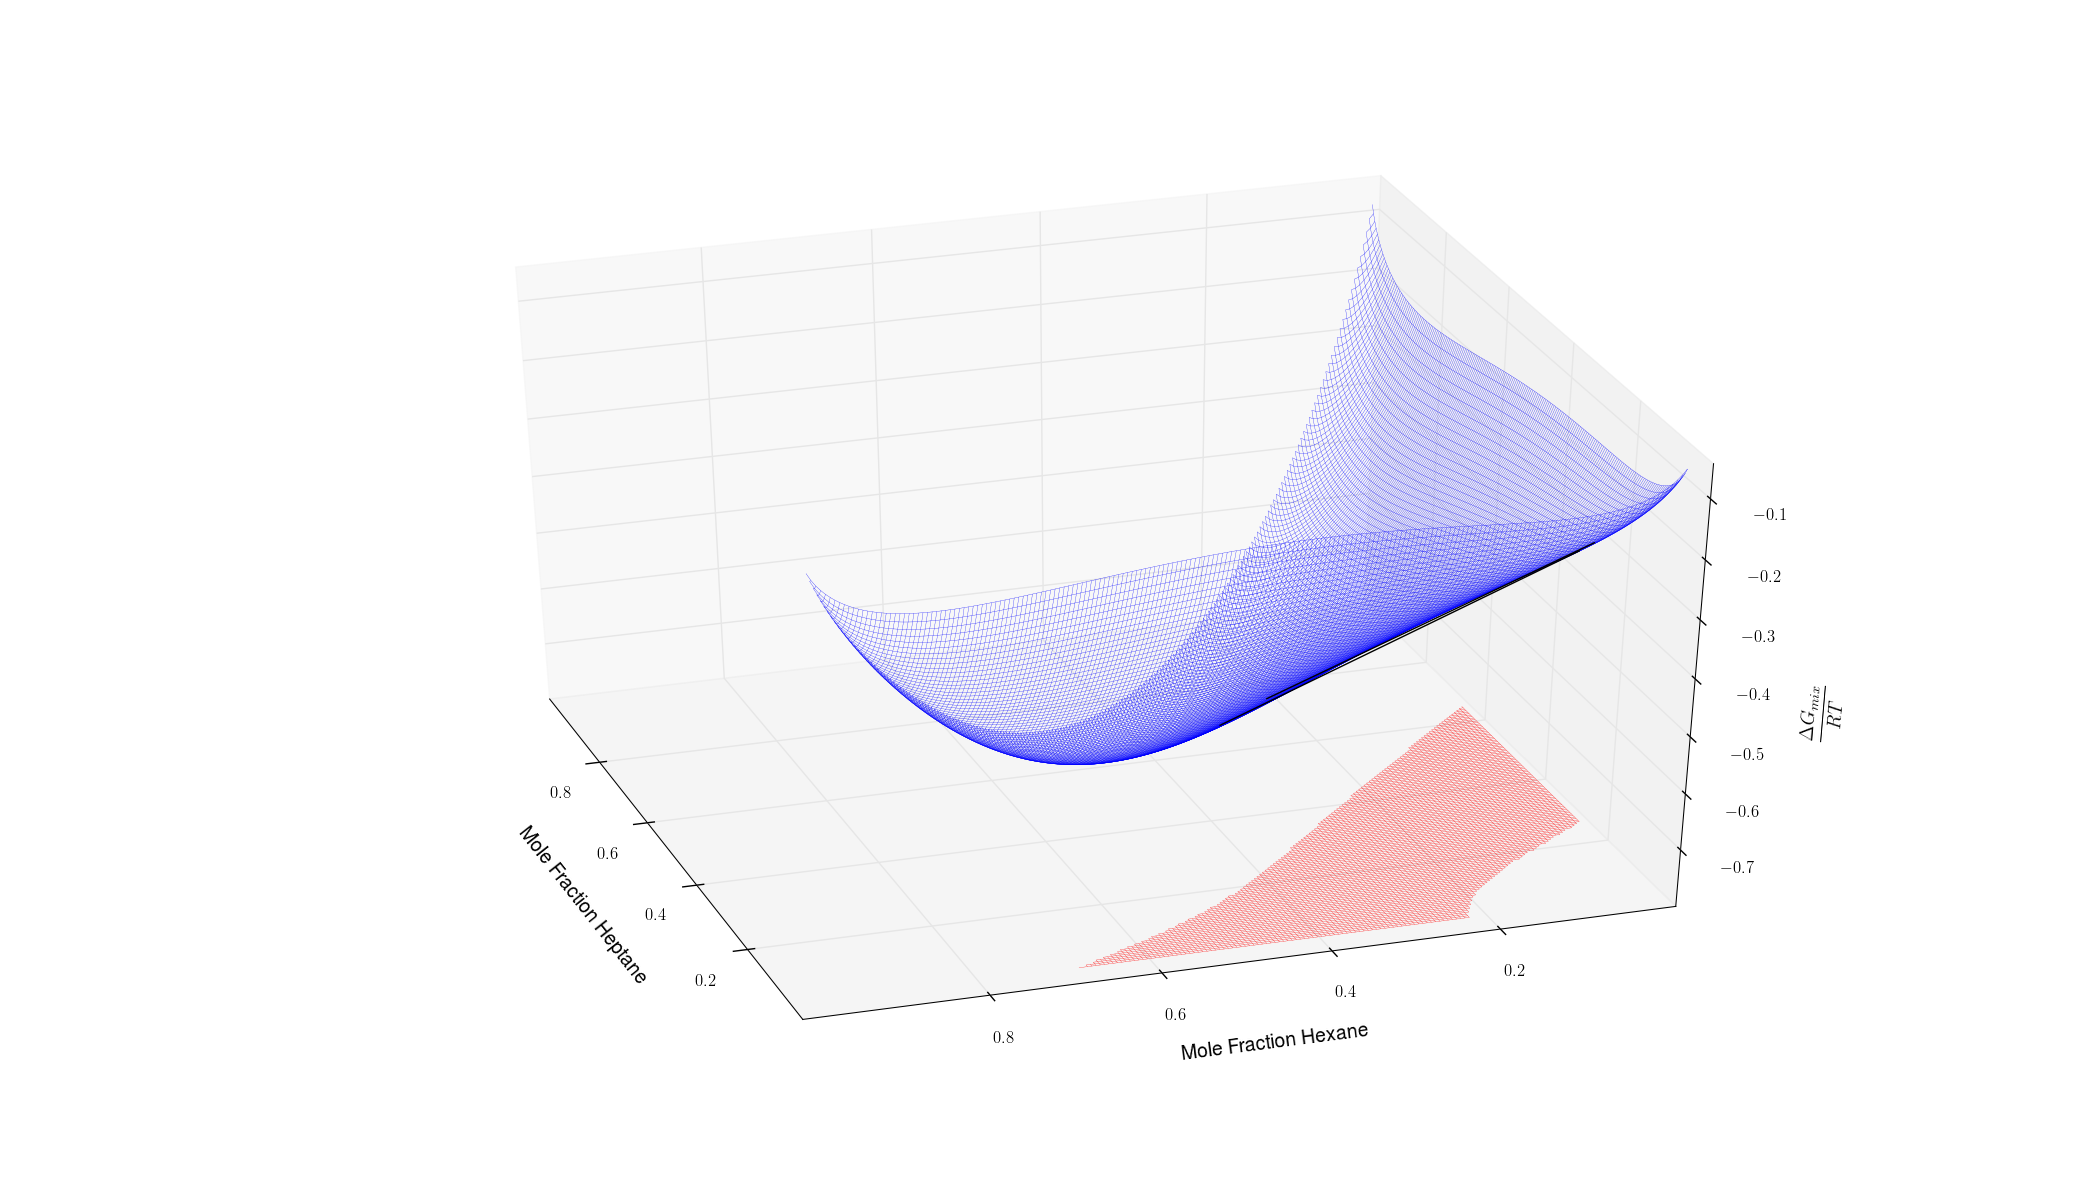
\includegraphics[width = \textwidth, bb=100 100 1600 700]{Results_Parts/TernaryParams/heptane-hexane-methanol/DWPMTieline3and4/rotation6.png}
\caption[]{(Continued) Rotated View 2}
\end{figure}

\begin{figure}[hp]
\vspace{40pt}
\ContinuedFloat
\centering
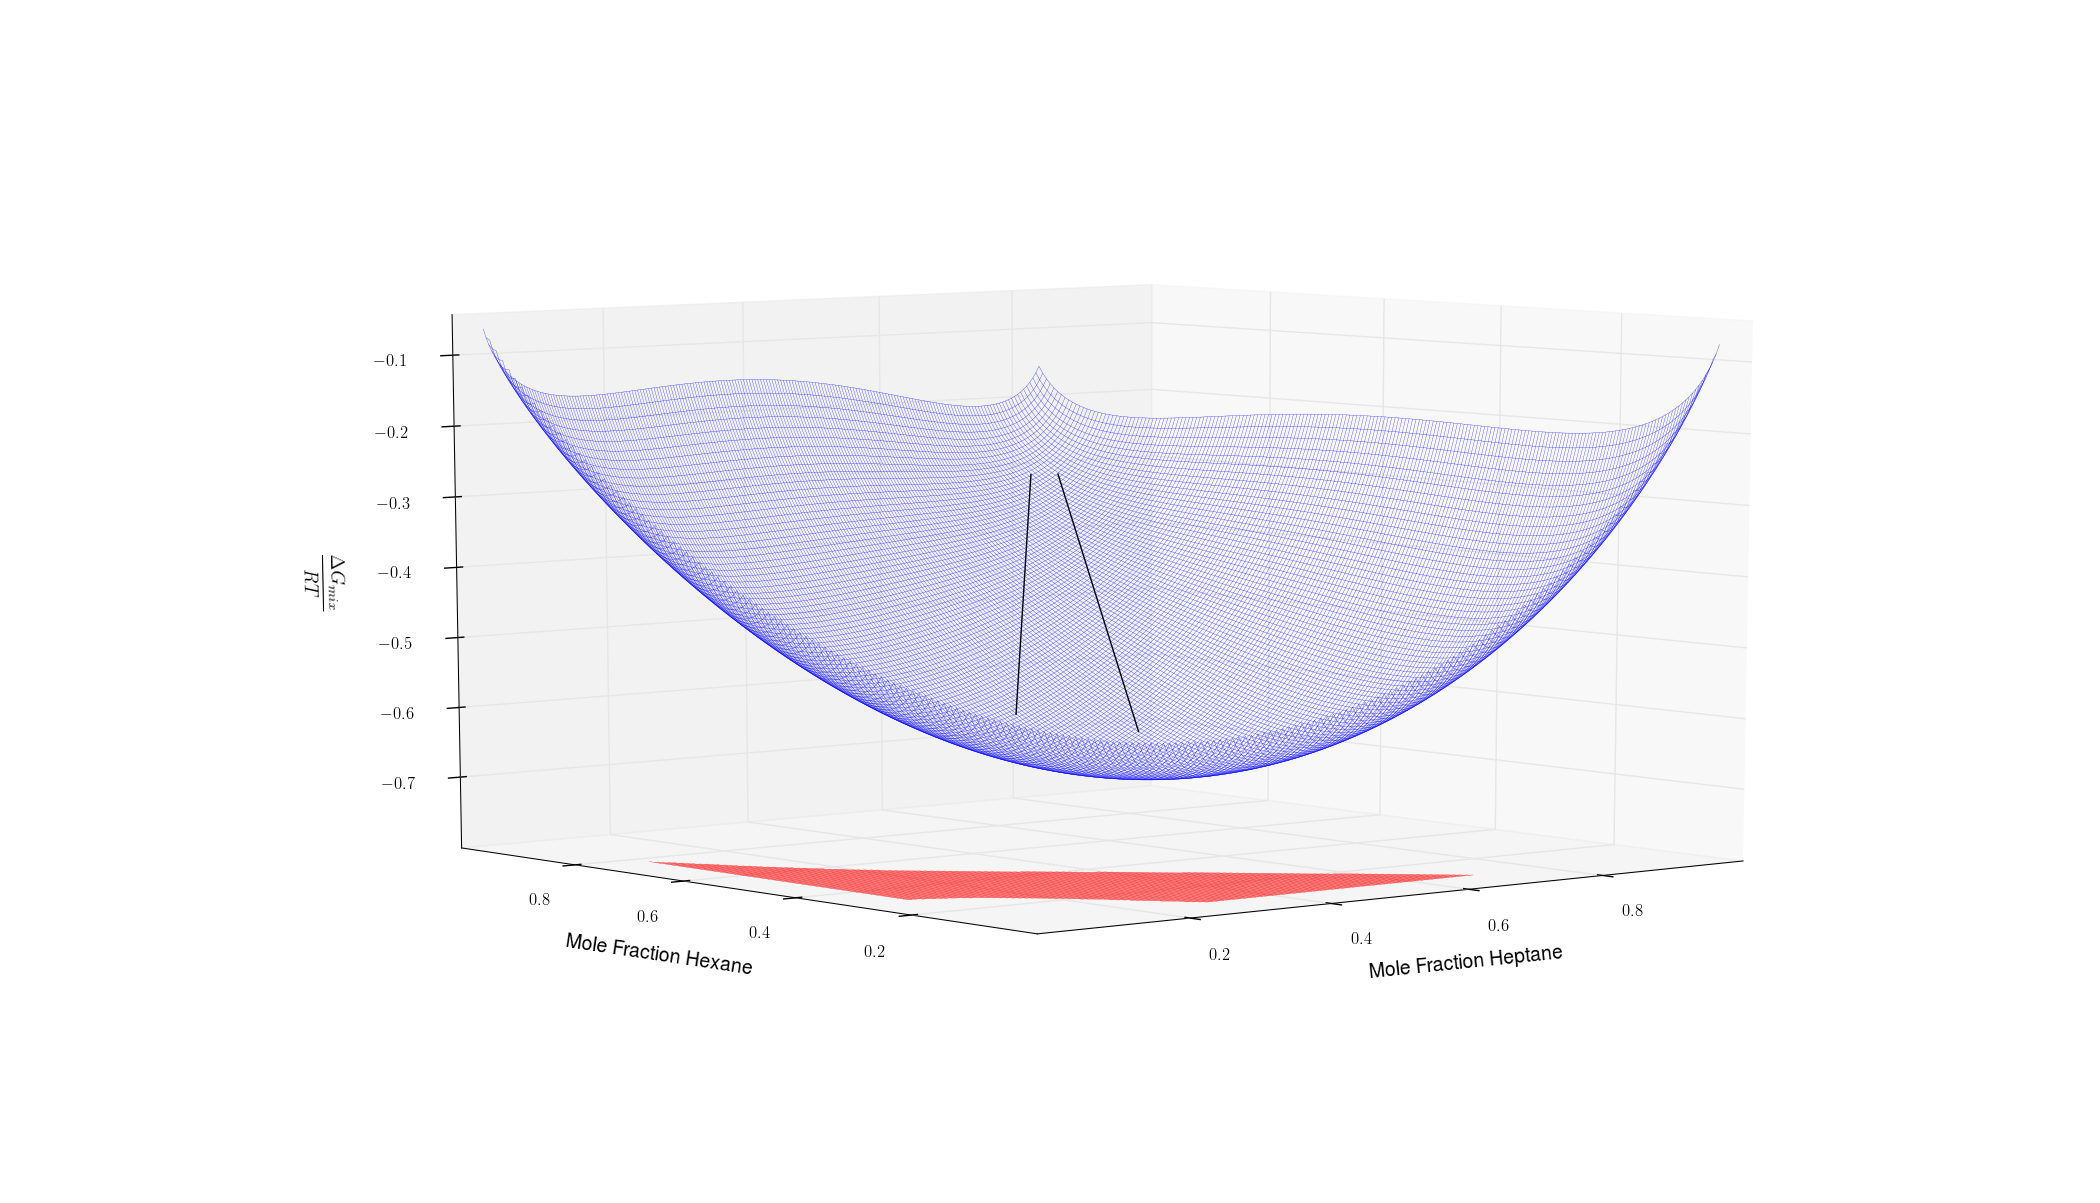
\includegraphics[width = \textwidth, bb=100 100 1600 700]{Results_Parts/TernaryParams/heptane-hexane-methanol/DWPMTieline3and4/rotation8.png}
\caption[]{(Continued) Rotated View 3}
\end{figure}

\clearpage

\begin{figure}[hp]
 \vspace{40pt}
\centering
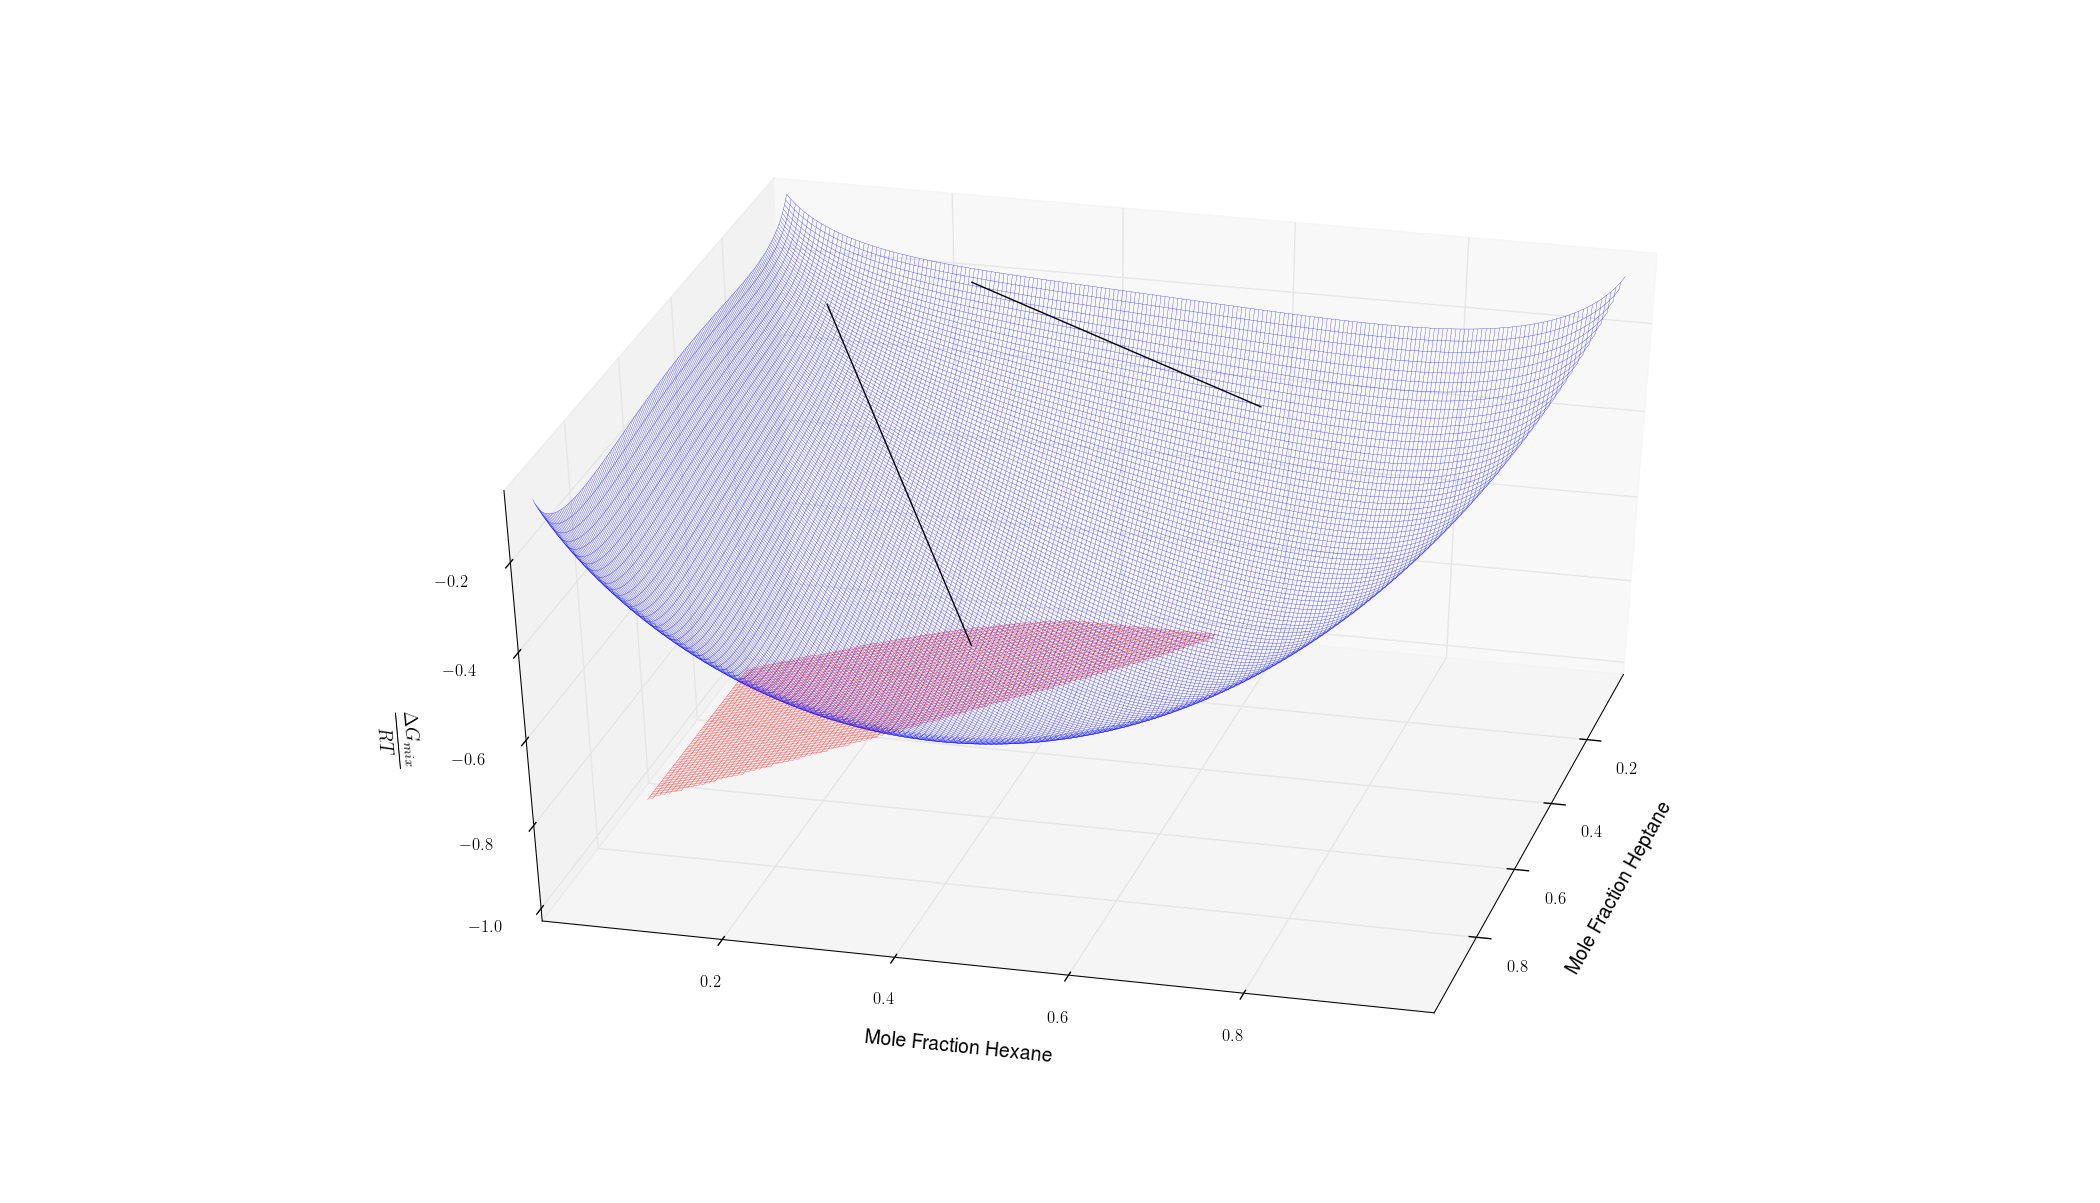
\includegraphics[width = \textwidth, bb=100 100 1600 700]{Results_Parts/TernaryParams/heptane-hexane-methanol/DWPMTieline3and-2/rotation6.png}
\caption{Predicted Gibbs energy surface for Heptane, Hexane and Methanol at $305.95~\mathrm{K}$, using parameters calculated from experimental tie-lines 3 and second to last.}
\end{figure}	

\begin{figure}[hp]
\vspace{40pt}
\ContinuedFloat
\centering
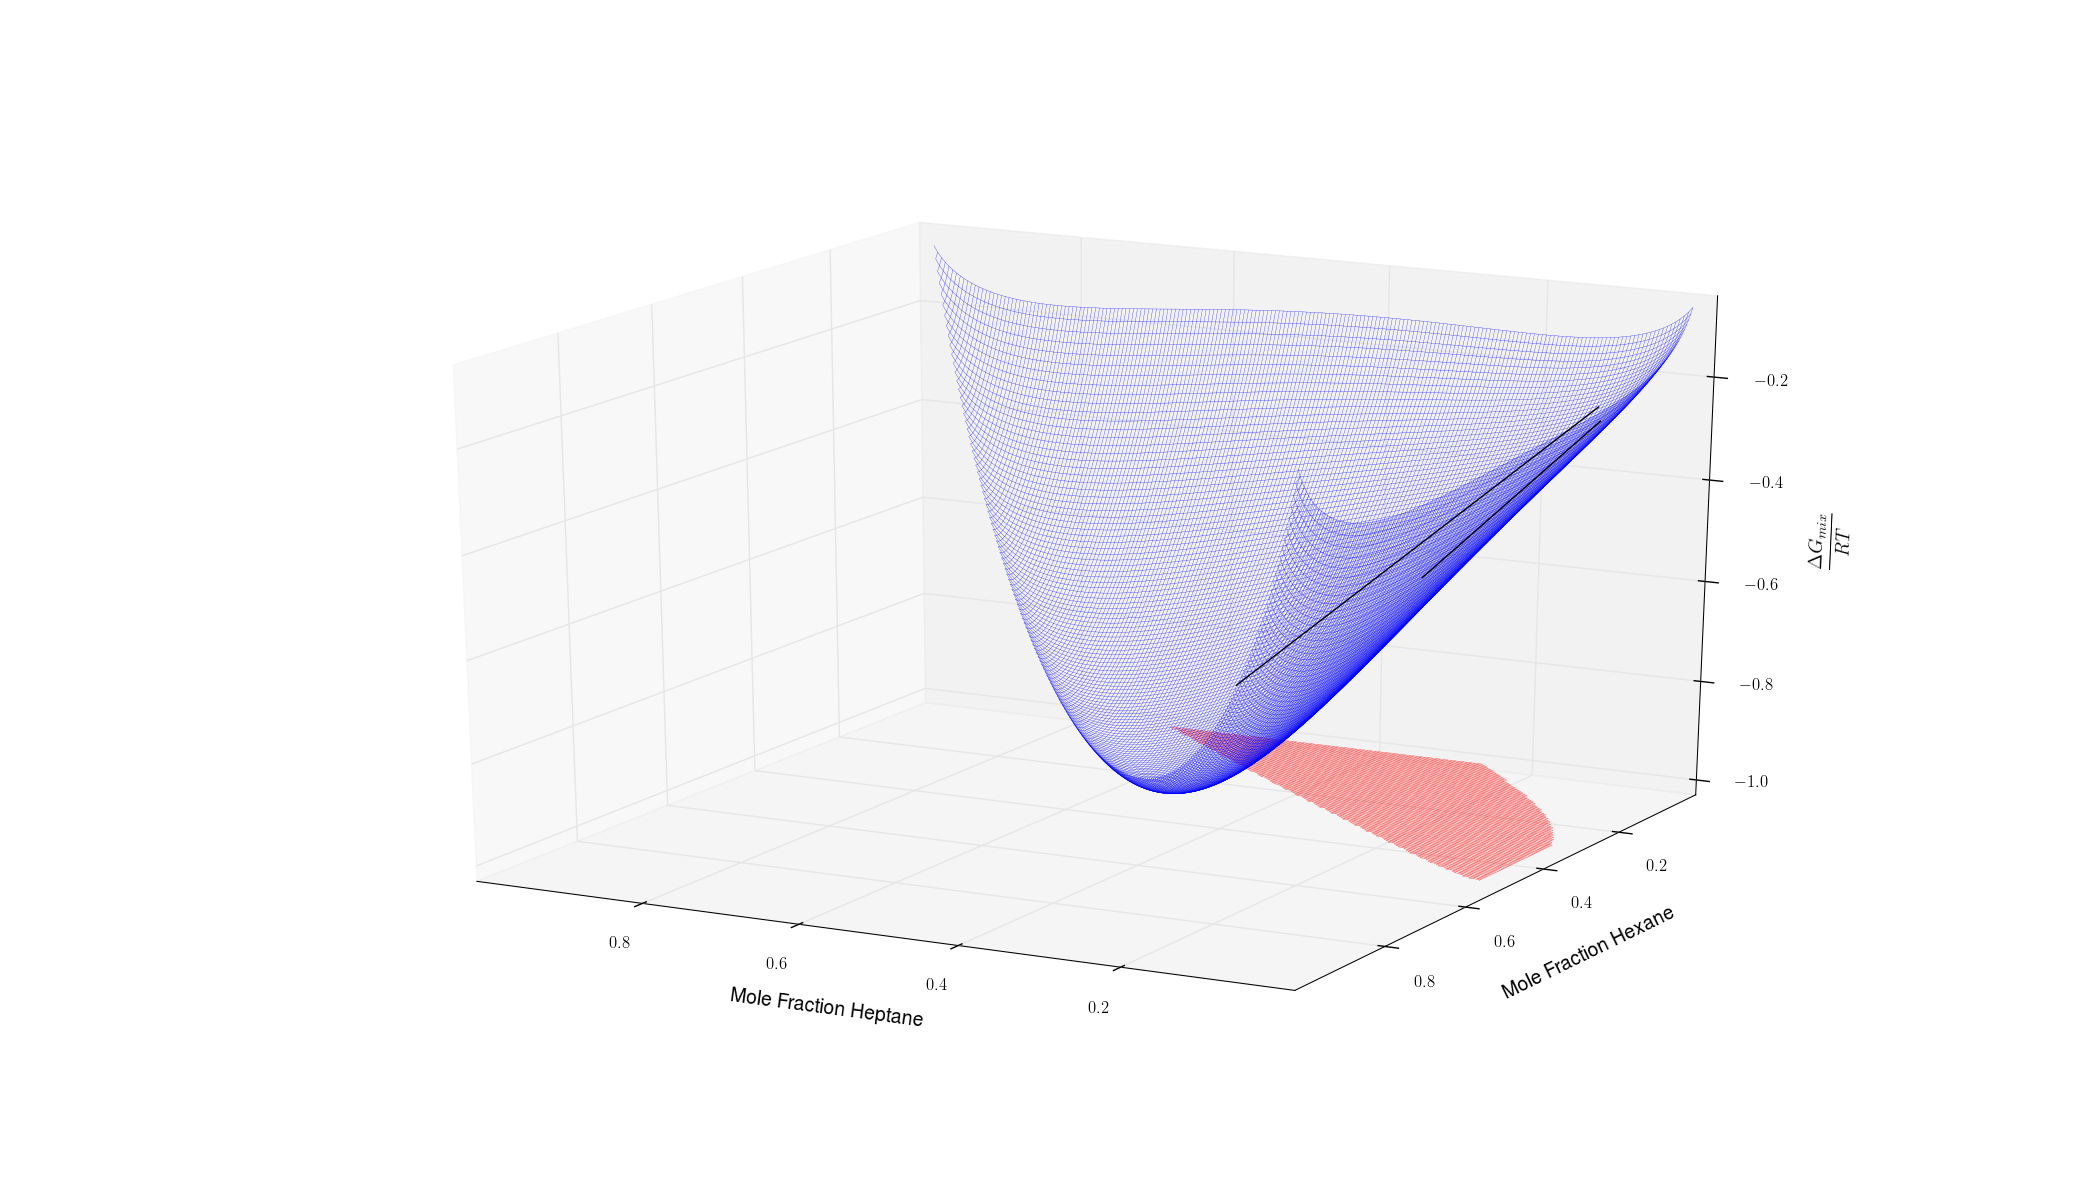
\includegraphics[width = \textwidth, bb=100 100 1600 700]{Results_Parts/TernaryParams/heptane-hexane-methanol/DWPMTieline3and-2/rotation2.png}
\caption[]{(Continued) Rotated View 1}
\end{figure}

\begin{figure}[hp]
\vspace{40pt}
\ContinuedFloat
\centering
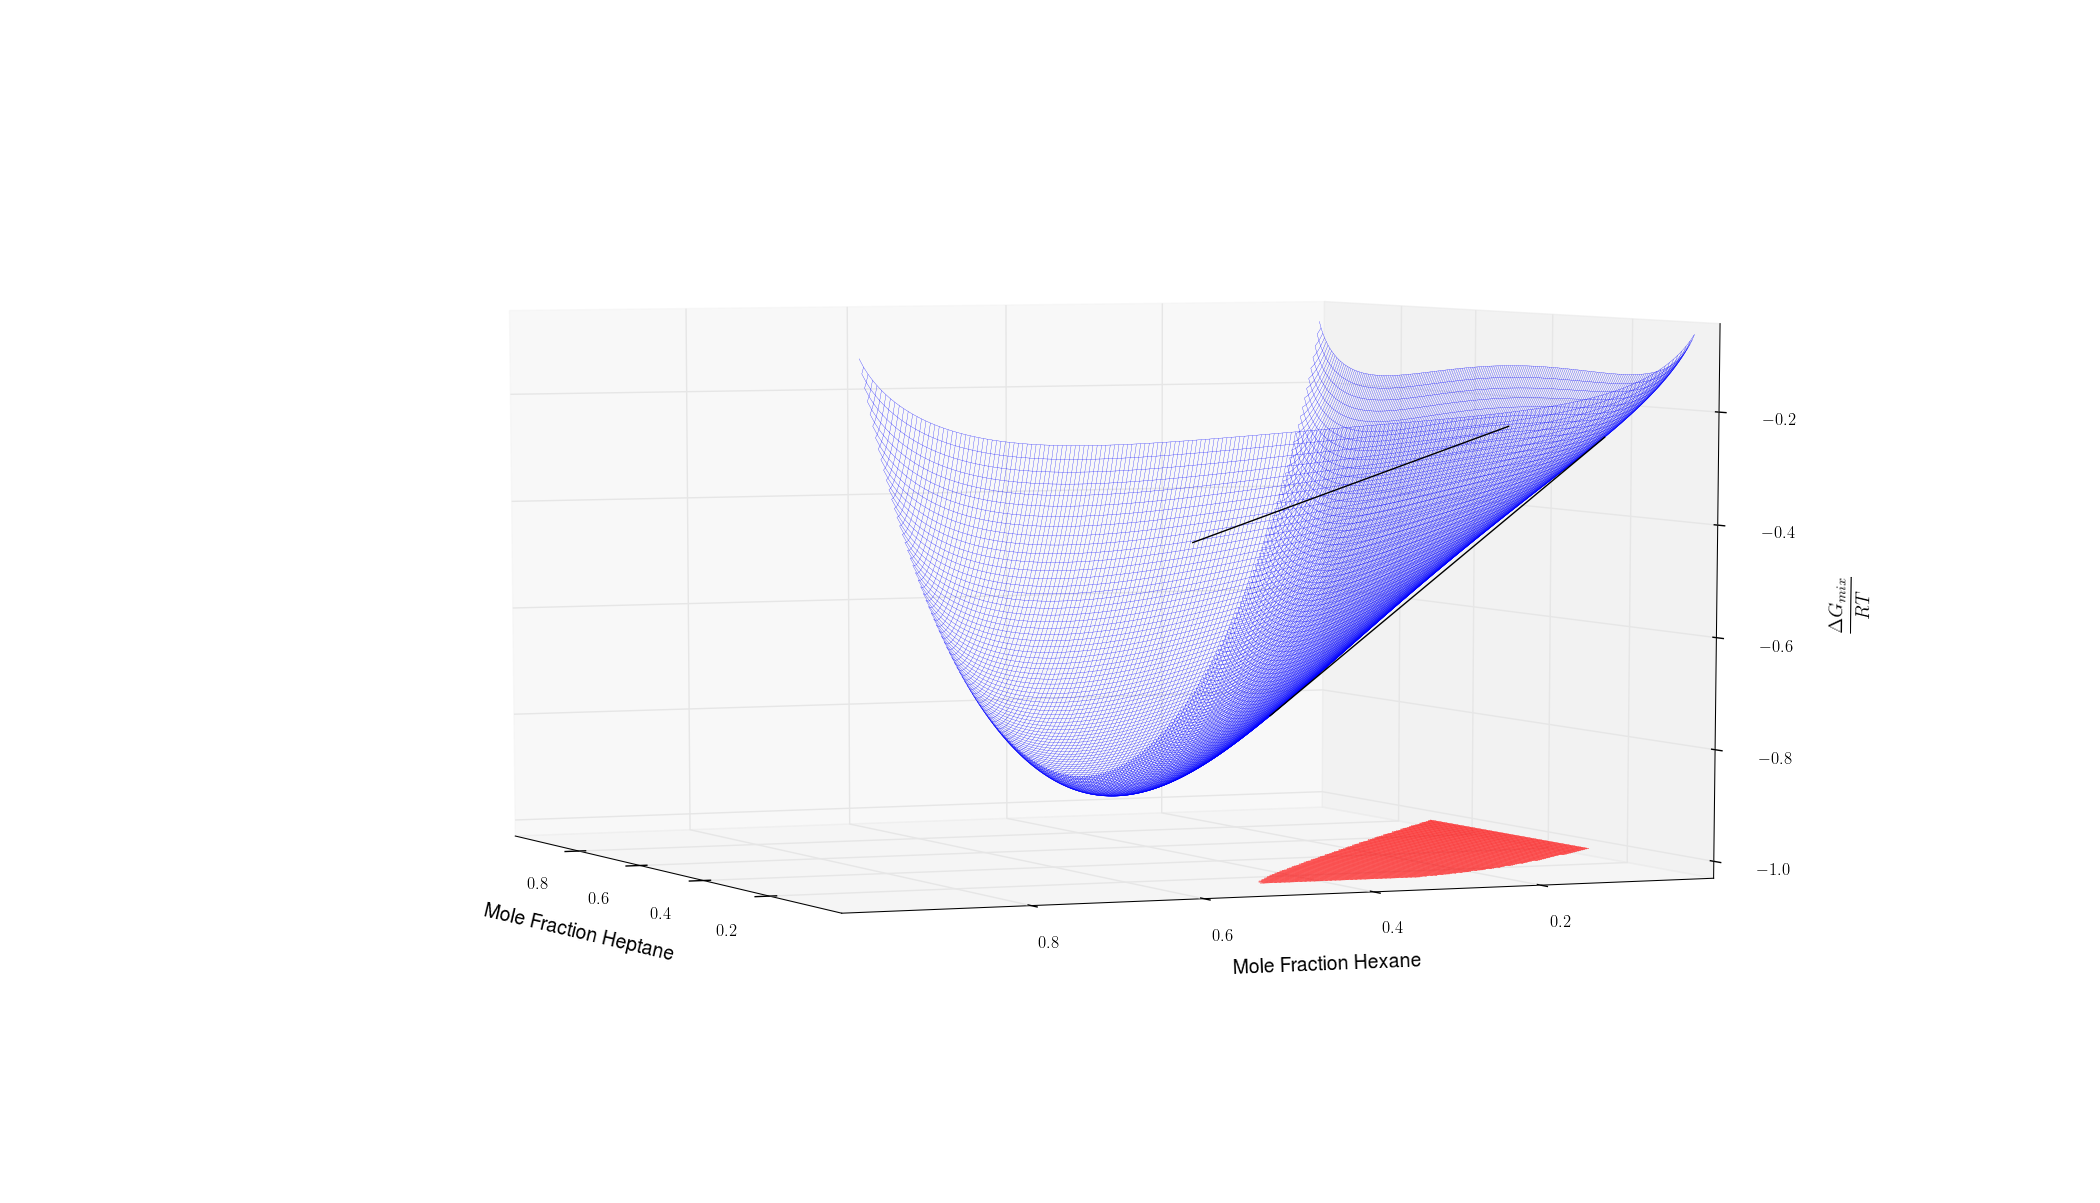
\includegraphics[width = \textwidth, bb=100 100 1600 700]{Results_Parts/TernaryParams/heptane-hexane-methanol/DWPMTieline3and-2/rotation4.png}
\caption[]{(Continued) Rotated View 2}
\end{figure}

\clearpage
%%------------------------------- 1-Hexanol, Nitro-Methane and Water-------------------------------------------%
\subsection{1-Hexanol, Nitro-Methane and Water}

\begin{figure}[hp]
\centering
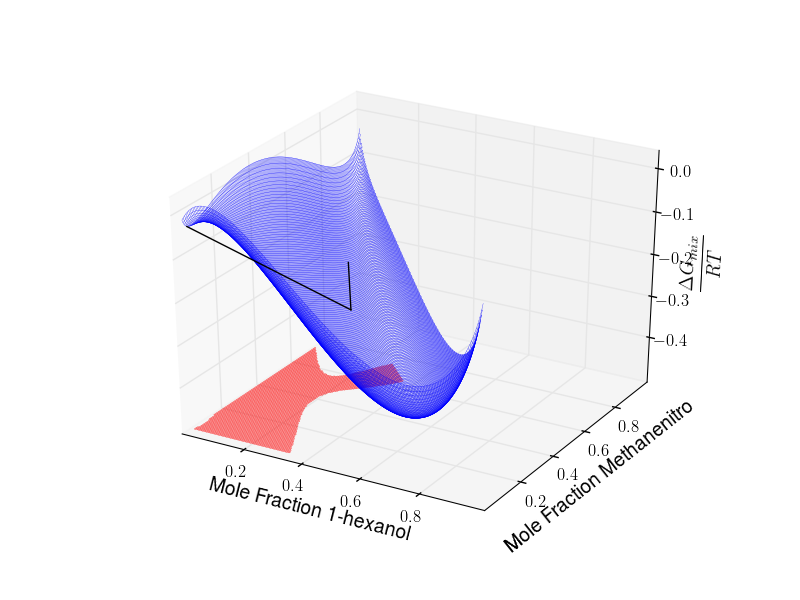
\includegraphics[width = 0.6\textwidth, bb=100 0 500 400]{Results_Parts/TernaryParams/1-hexanol-methanenitro-water/DWPM/294.15/PredictedGibbsWireframe.png}
\caption{Predicted Gibbs energy surface for 1-Hexanol, Nitro-Methane and Water at $294.15~\mathrm{K}$.}
\end{figure}	


\begin{figure}[hp]
\centering
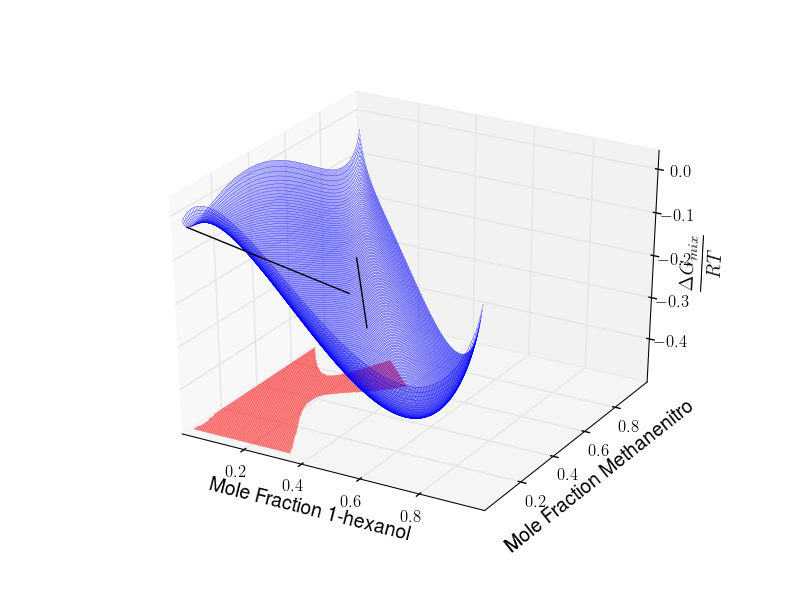
\includegraphics[width = 0.6\textwidth, bb=100 0 500 400]{Results_Parts/TernaryParams/1-hexanol-methanenitro-water/DWPM/296.15/PredictedGibbsWireframe.png}
\caption{Predicted Gibbs energy surface for 1-Hexanol, Nitro-Methane and Water at $296.15~\mathrm{K}$.}
\end{figure}

